\begin{figure}[t]
    \centering
    \begin{minipage}[t]{0.8\linewidth}
        
\includegraphics[width=0.99\linewidth]{chapters/robust/figures/new_legend.pdf}
        \end{minipage}
    \begin{minipage}[t]{\linewidth}
        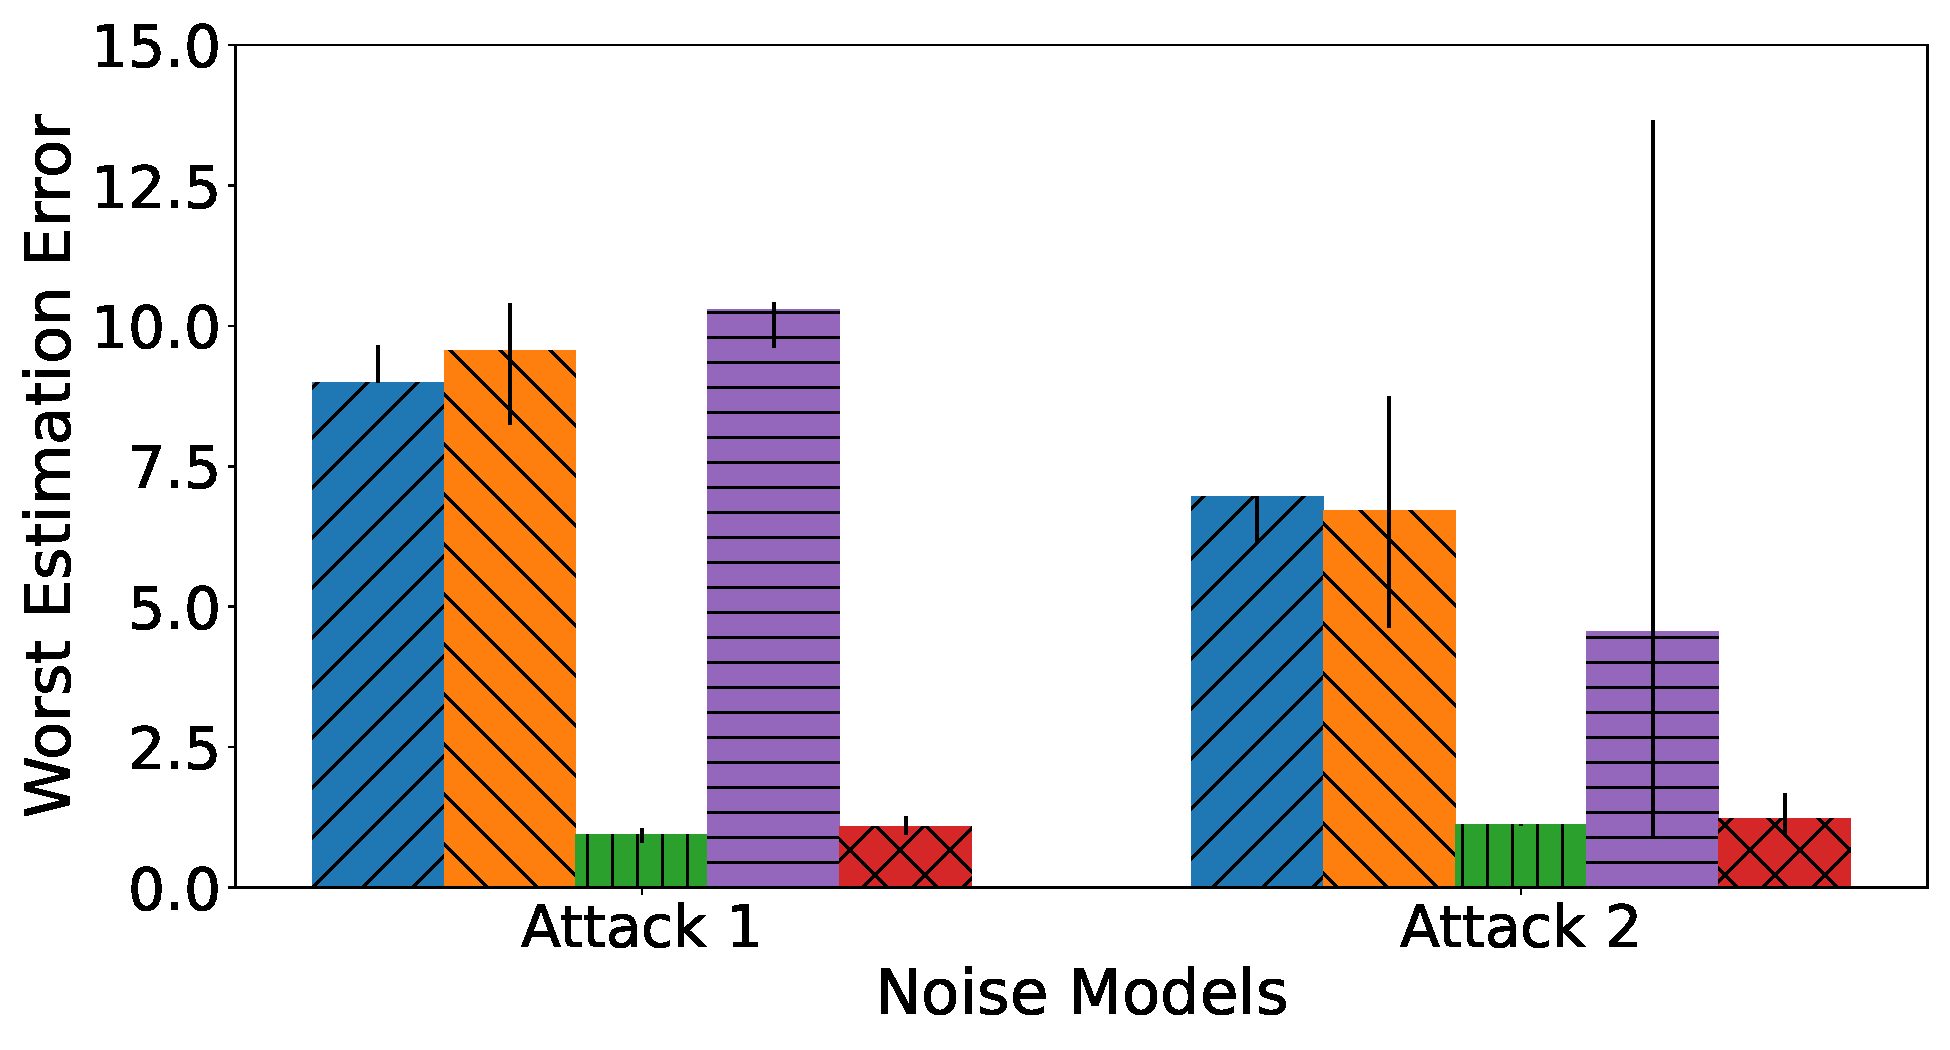
\includegraphics[width=0.49\linewidth]{chapters/robust/figures/gauss_inliers_2_attacks_error.pdf}
        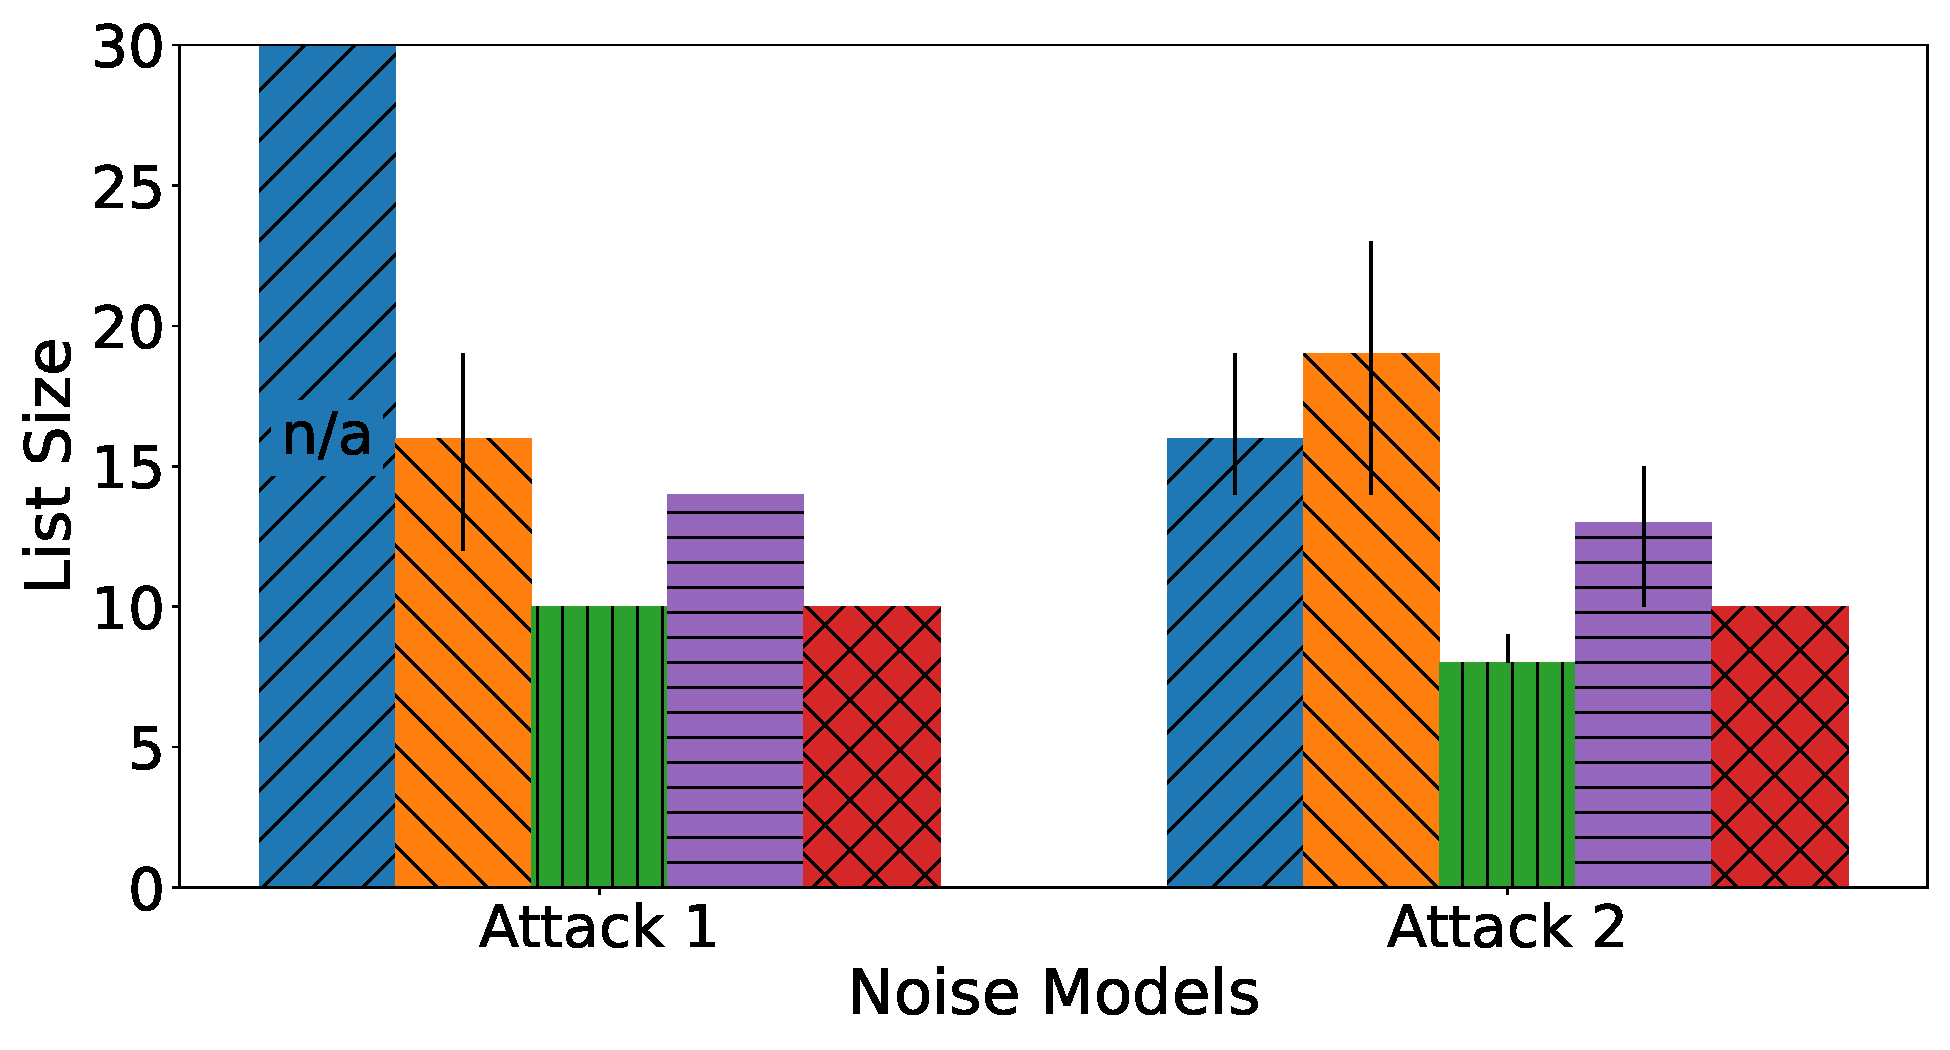
\includegraphics[width=0.49\linewidth]{chapters/robust/figures/gauss_inliers_2_attacks_size.pdf}
    \end{minipage}
    \caption{
    Comparison of five algorithms with two adversarial noise models. The attack distributions and further experimental details are given in~\Cref{app:exp-details}. On the left we show worst estimation error for constrained list size and on the right the smallest list size for constrained error guarantee.
    We plot the median of the metrics with the error bars showing \(25\)th and \(75\)th percentile.
    }
    \label{fig:list_size}
\end{figure}
\vspace{-0.1in}
\section{Discussion and future work}
\label{sec:exp}


In this work, we prove that even when small groups are outnumbered by adversarial data points, efficient list-decodable algorithms can provide an accurate estimation of all means with minimal list size. 
The proof for the upper bound is constructive and analyzes a plug-and-play meta-algorithm  (cf.~\Cref{fig:alg_diagram}) that inherits guarantees of the black-box $\ckLD$ algorithm $\ckLDA$ and $\rme$ algorithm $\cA_R$, which it uses as base learners. 
Notably, when the inlier mixture is a mixture of Gaussians with identity covariance, we achieve optimality.
Furthermore, any new development for the base learners
automatically translates to improvements in our bounds.

We would like to end by discussing the possible practical impact of this result. 
Since an extensive empirical study is out of the scope of this paper, 
besides the fact that ground-truth means for unsupervised real-world data are hard to come by, we provide preliminary experiments on synthetic data.
Specifically, we generate data from a separated $k-$Gaussian mixture with additive contaminations as in~\Cref{eq:gen_model} and different types of adversarial distributions (see detailed description in~\Cref{app:exp-details}). We focus on the regime
$\epsilon \sim w_i$ where our algorithms shows the largest theoretical improvements. Precisely, we consider \(k = 7\) inlier clusters in \(d = 100\) dimensions with cluster weights ranging from \(0.3\) to \(0.02\), \(\wmin = 0.02\), and \(\epsilon = 0.12\).
We implement our meta-algorithm with the LD-ME base learner from~\cite{diakonikolas2022clustering} (omitting the RME base learner improvement for large clusters). 

We then compare the output of our algorithm with the vanilla LD-ME algorithm from~\cite{diakonikolas2022clustering} with $\wmin=0.02$ and (suboptimal) LD-ML guarantees as well as
well-known (robust) clustering heuristics without LD-ML guarantees,
such as the $k$-means~\citep{lloyd1982least}, Robust $k$-means~\citep{brownlees2015empirical}, and DBSCAN~\citep{ester1996density}. 
Even though none of these heuristics  have LD-ML guarantees, they are commonly used and known to also perform well in practice in noisy settings. The hyper-parameters of the algorithms are tuned beforehand and for the comparative algorithms multiple tuned configurations are selected for the experiments.
For each algorithm, we run \(100\) seeds of each parameter setting and record their performance. 
In~\Cref{fig:list_size} (left), we fix the list size to \(10\) and plot the errors for the worst inlier cluster, typically the smallest. 
We compare the performance of the algorithms by plotting the worst-case estimation errors for a given list size and list sizes that each algorithm requires to achieve a given worst-case estimation error.
In~\Cref{fig:list_size} (right), we fix the error and plot the minimal list size at which competing algorithms reach the same or smaller worst estimation error. Further details on the evaluation metric and parameter tuning are provided in~\Cref{app:exp-details}.

In a different experiment (see~\Cref{sec:app-wlow} for details), we study the effect of varying \(\wmin\) on the performance of our approach and LD-ME.~\Cref{fig:wlow_variation_short} shows the worst estimation error for a cluster with weight of \(0.2\) that is contaminated by noise. As expected from our theoretical results, we observe that the mean-estimation performance of our algorithm stays roughly constant, regardless of the initial \(\wmin\). Meanwhile, the estimation error of LD-ME increases as \(\wmin\) decreases further below  the true cluster weight. 
Furthermore, our algorithm consistently outperforms LD-ME in both estimation error and list size, demonstrating significantly lower list size values with only a slight decrease in the same. 

\begin{figure}[t]
    \centering
    \begin{minipage}[t]{\linewidth}
        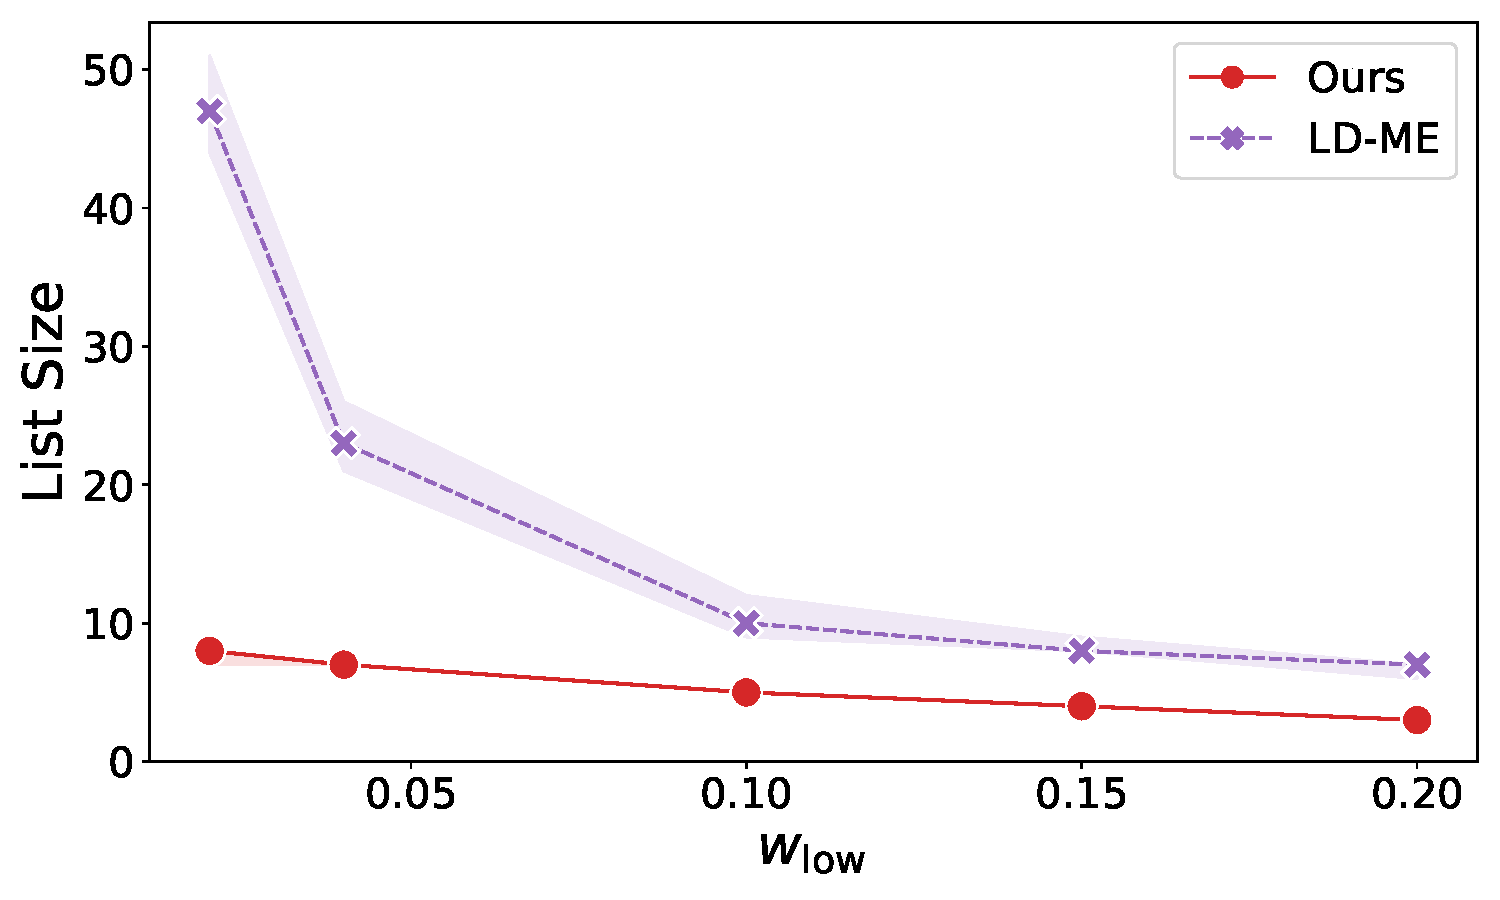
\includegraphics[width=0.49\linewidth]
        {chapters/robust/figures/wlow_variation_size.pdf}
        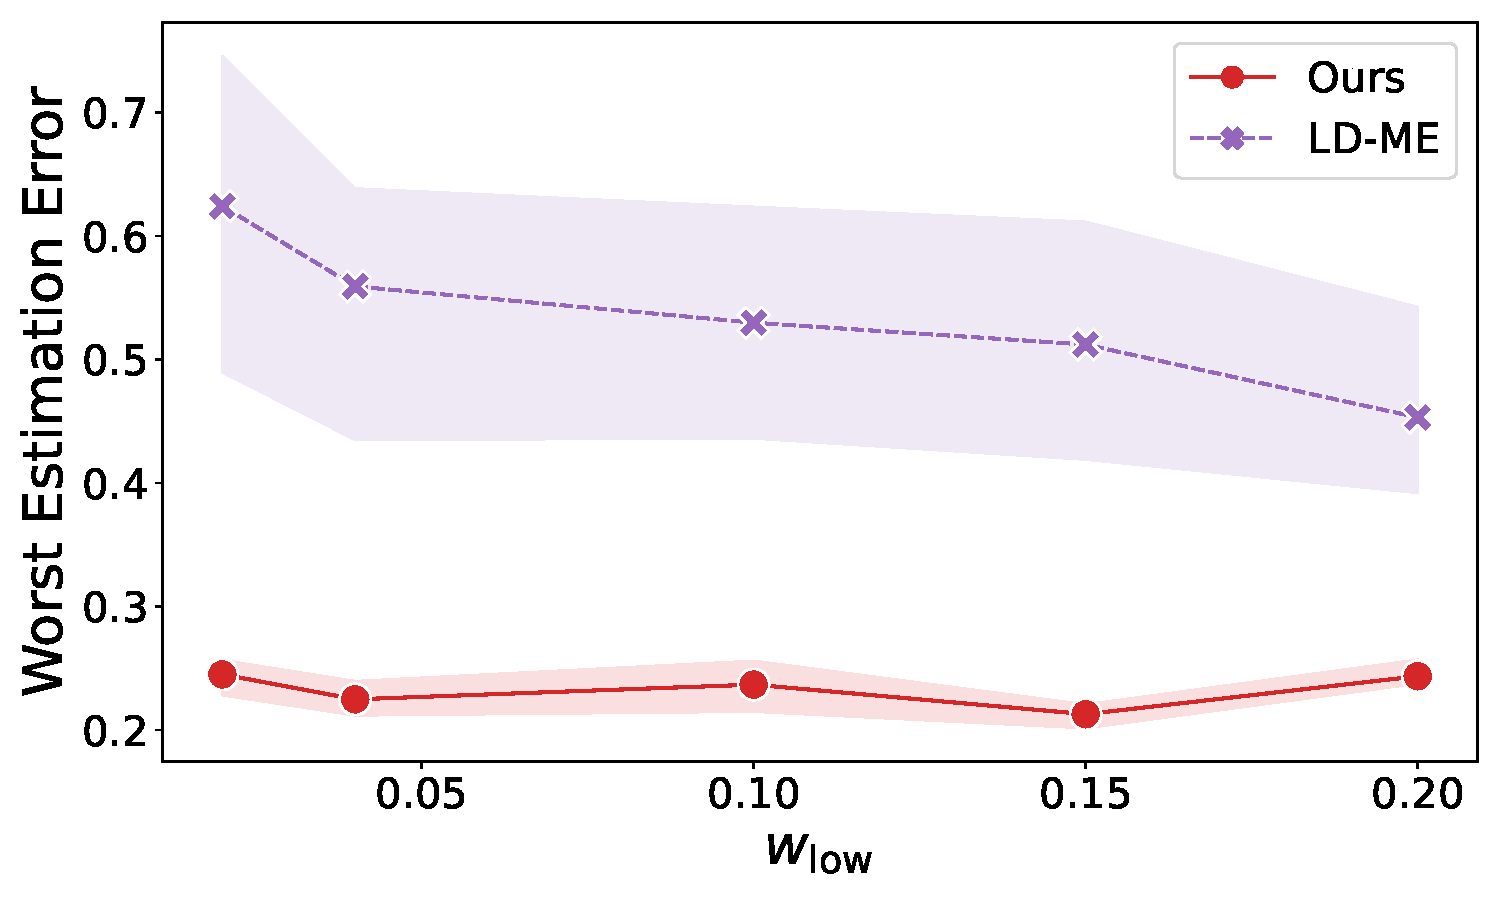
\includegraphics[width=0.49\linewidth]{chapters/robust/figures/wlow_variation_error_large.pdf}
    \end{minipage}
    \caption{Comparison of list size and estimation error for large inlier cluster for varying \(\wmin\) inputs. The experimental setup is illustrated in~\Cref{app:exp-details}. We plot the median values with error bars showing \(25\)th and \(75\)th quantiles. As \(\wmin\) decreases, we observe a roughly constant estimation error for our algorithm while the error for LD-ME increases. Further, the decrease in list size is much more severe for LD-ME than for our algorithm.}
    \label{fig:wlow_variation_short}
\end{figure}

Overall, we observe that, in line with our theory, our method significantly outperforms the LD-ME algorithm, and performs better or on par with the heuristic approaches. Additional experimental comparison and implementation details can be found in~\Cref{app:exp-details}. Even though these experiments do not allow conclusive statements about the improvement of our algorithm for mixture learning for real-world data, they do provide encouraging evidence that effort could be well-spent on follow-up empirical and theoretical work building on our results. 
For example, it would be interesting to conduct a more extensive empirical study that compares our algorithm against a plethora of robust clustering algorithms. 
Furthermore, practical data often includes components with different covariances and scalings. One could hence explore an extension of our algorithm that can incorporate different covariances at the same time being agnostic to it. 
